\documentclass[12pt]{article}
\usepackage[paper=letterpaper,margin=2cm]{geometry}
\usepackage{amsmath,amssymb,amsfonts}
\usepackage{enumitem}
\usepackage{titling}
\usepackage{multirow}
\usepackage{xcolor}
\usepackage{float}
\usepackage{graphicx}
\usepackage{xcolor}
\definecolor{ISTBlue}{RGB}{0, 139, 255}
\usepackage[colorlinks=true, linkcolor=red]{hyperref}
\usepackage{subcaption} % For subfigures
\usepackage{adjustbox}  % For centering the bottom image
\usepackage{listings}
\usepackage{xcolor} % For setting colors
\usepackage{booktabs} % For better tables
\usepackage{threeparttable} % For table notes

\usepackage{listings}
\usepackage{xcolor}

\definecolor{codegreen}{rgb}{0.0, 0.514, 0.325}      
\definecolor{codegray}{rgb}{0.75, 0.75, 0.75}    
\definecolor{codeblue}{rgb}{0.122, 0.467, 0.706}  
\definecolor{extraLightGray}{rgb}{0.98, 0.98, 0.98}
\definecolor{codepink}{rgb}{0.894, 0.0, 0.443}

\lstdefinestyle{mystyle}{
    backgroundcolor=\color{extraLightGray},
    commentstyle=\color{codegreen},
    keywordstyle=\color{codeblue},
    numberstyle=\tiny\color{codegray},
    stringstyle=\color{codepink},
    basicstyle=\ttfamily\footnotesize,
    breakatwhitespace=false,
    breaklines=true,
    captionpos=b,
    keepspaces=true,
    numbers=left,
    numbersep=5pt,
    showspaces=false,
    showstringspaces=false,
    showtabs=false,
    tabsize=2
}
\lstset{style=mystyle}

\setlength{\droptitle}{-6em}

\begin{document}

\begin{center}
Aprendizagem 2023\\
Homework I --- Group 003\\
(ist1107028, ist1107137)\vskip 1cm
\end{center}

\large{\textbf{Part I}: Pen and paper}\normalsize

\vspace{20pt}
\hspace{-20pt}\textbf{We collected four positive (P) observations,}
\[
\boldsymbol{\{x_1 = (A,0), \quad x_2 = (B,1), \quad x_3 = (A,1), \quad x_4 = (A,0)\}}
\]
\textbf{and four negative (N) observations,}
\[
\boldsymbol{\{x_5 = (B,0), \quad x_6 = (B,0), \quad x_7 = (A,1), \quad x_8 = (B,1)\}}
\]


\hspace{-20pt}\textbf{Consider the problem of classifying observations as positive or negative.}

\vspace{10pt}
\begin{enumerate}[leftmargin=\labelsep]
    \item \textbf{Compute the F1-measure of a $\mathbf{k}$NN with $\mathbf{k =  5}$ and Hamming distance using a
    leave-one-out evaluation schema. Show all calculus.}

    \vspace{10pt}
    We start by calculating Hamming distance between observations. The Hamming distance is the number of positions at which the corresponding symbols are different.\\
    Since we are workin with $k = 5$, we will consider the 5 nearest neighbors of each observation (written in blue).
    \vspace{10pt}
    
    \begin{table}[H]
        \begin{center}
            \begin{tabular}{c|cccccccc}
            & $x_1$ & $x_2$ & $x_3$ & $x_4$ & $x_5$ & $x_6$ & $x_7$ & $x_8$\\ 
            \hline
                $x_1$ & \-- & 2 & \textbf{\textcolor{codeblue}{1}} & \textbf{\textcolor{codeblue}{0}} & \textbf{\textcolor{codeblue}{1}} & \textbf{\textcolor{codeblue}{1}} & \textbf{\textcolor{codeblue}{1}} & 2 \\ 
                $x_2$ & 2 & \-- & \textbf{\textcolor{codeblue}{1}} & 2 & \textbf{\textcolor{codeblue}{1}} & \textbf{\textcolor{codeblue}{1}} & \textbf{\textcolor{codeblue}{1}} & \textbf{\textcolor{codeblue}{0}} \\ 
                $x_3$ & \textbf{\textcolor{codeblue}{1}} & \textbf{\textcolor{codeblue}{1}} & \-- & \textbf{\textcolor{codeblue}{1}} & 2 & 2 & \textbf{\textcolor{codeblue}{0}} & \textbf{\textcolor{codeblue}{1}} \\ 
                $x_4$ & \textbf{\textcolor{codeblue}{0}} & 2 & \textbf{\textcolor{codeblue}{1}} & \-- & \textbf{\textcolor{codeblue}{1}} & \textbf{\textcolor{codeblue}{1}} & \textbf{\textcolor{codeblue}{1}} & 2 \\ 
                $x_5$ & \textbf{\textcolor{codeblue}{1}} & \textbf{\textcolor{codeblue}{1}} & 2 & \textbf{\textcolor{codeblue}{1}} & \-- & \textbf{\textcolor{codeblue}{0}} & 2 & \textbf{\textcolor{codeblue}{1}} \\ 
                $x_6$ & \textbf{\textcolor{codeblue}{1}} & \textbf{\textcolor{codeblue}{1}} & 2 & \textbf{\textcolor{codeblue}{1}} & \textbf{\textcolor{codeblue}{0}} & \-- & 2 & \textbf{\textcolor{codeblue}{1}} \\ 
                $x_7$ & \textbf{\textcolor{codeblue}{1}} & \textbf{\textcolor{codeblue}{1}} & \textbf{\textcolor{codeblue}{0}} & \textbf{\textcolor{codeblue}{1}} & 2 & 2 & \-- & \textbf{\textcolor{codeblue}{1}} \\ 
                $x_8$ & 2 & \textbf{\textcolor{codeblue}{0}} & \textbf{\textcolor{codeblue}{1}} & 2 & \textbf{\textcolor{codeblue}{1}} & \textbf{\textcolor{codeblue}{1}} & \textbf{\textcolor{codeblue}{1}} & \-- \\ 
            \end{tabular}
            \caption{Hamming distance between observations}
        \end{center}
    \end{table}

    Now that we have the Hamming distance between all observations, we must identify if the prediction is correct or not. We will consider the majority class of the 5 nearest neighbors for each observation.
    
    \vspace{10pt}
    \underline{Example}: For $x_1$, the 5 nearest neighbors are $x_3$ and $x_4$ (which are positive), $x_5$, $x_6$ and $x_7$ (which are negative). The majority class is negative, therefore the prediction is incorrect.
    
    \newpage
    We apply the same logic for the rest of the classes, ending up with the following table:

    \begin{table}[H]
        \begin{center}
            \begin{threeparttable}
            \begin{tabular}{c|c|c|c}
                Observation & True Value & Prediction & Confusion Matrix Terminology\\
                \hline
                $x_1$ & P & N & FN\\
                $x_2$ & P & N & FN\\
                $x_3$ & P & P & TP\\
                $x_4$ & P & N & FN\\
                $x_5$ & N & P & FP\\
                $x_6$ & N & P & FP\\
                $x_7$ & N & P & FP\\
                $x_8$ & N & N & TN\\
            \end{tabular}
            \begin{tablenotes}
                \small
                \item[]
                \item[P - Positive observation; N - Negative observation]  
                \item[TP - True Positive; TN - True Negative; FP - False Positive; FN - False Negative] 
                \item[] 
            \end{tablenotes}
        \end{threeparttable}
            \caption{Predictions for each observation - $k=5$}
        \end{center}
    \end{table}

    With this table, we can know calculate the Precision, Recall and F1-measure using the following formulas:

    \begin{equation}\label{precision}
        \text{Precision} = \frac{\text{True Positives}}{{\text{True Positives} +
        \text{False Positives}}}
    \end{equation}

    \begin{equation}\label{recall}
        \text{Recall} = \frac{\text{True Positives}}{{\text{True Positives} + \text{False Negatives}}}
    \end{equation}

    \begin{equation}\label{f1}
        \text{F1-measure} = 2 \times \frac{{\text{Precision} \times \text{Recall}}}{{\text{Precision} + \text{Recall}}}
    \end{equation}

    \vspace{10pt}
    Replacing the corresponding values in the formulas, we get:

    \vspace{10pt}
    for Precision \eqref{precision} and Recall \eqref{recall}:

    \begin{equation*}
        \text{Precision} = \frac{1}{1 + 3} = 0.25 \quad \quad
        \text{Recall} = \frac{1}{1 + 3} = 0.25
    \end{equation*}

    F1-measure \eqref{f1}:

    \begin{equation*}
        \text{F1-measure} = 2 \times \frac{0.25 \times 0.25}{0.25 + 0.25} = 0.25
    \end{equation*}

    \newpage
    \item \textbf{Propose a new metric (distance) that improves the latter's performance (i.e., the
    F1-measure) by three fold.} 
    
    \vspace{10pt}
    
    To improve the F1-measure, we propose using $K=3$ instead of $k=5$. This way, we will consider the 3 nearest neighbors of each observation.\\
    Simply by looking at the Hamming distance table, we can produce a new prediton table, like in the first exercise:

    \begin{table}[H]
        \begin{center}
            \begin{threeparttable}
            \begin{tabular}{c|c|c|c}
                Observation & True Value & Prediction & Confusion Matrix Terminology\\
                \hline
                $x_1$ & P & P & TP\\
                $x_2$ & P & N & FN\\
                $x_3$ & P & N & FN\\
                $x_4$ & P & P & TP\\
                $x_5$ & N & N & TN\\
                $x_6$ & N & N & TN\\
                $x_7$ & N & P & FP\\
                $x_8$ & N & P & FP\\
            \end{tabular}
            \begin{tablenotes}
                \small
                \item[]
                \item[P - Positive observation; N - Negative observation]  
                \item[TP - True Positive; TN - True Negative; FP - False Positive; FN - False Negative] 
                \item[] 
            \end{tablenotes}
        \end{threeparttable}
            \caption{Predictions for each observation - $k=3$}
        \end{center}
    \end{table}
    
    \begin{equation*}
        \text{Precision} = \frac{2}{2 + 2} =  0.5 \quad \quad
        \text{Recall} = \frac{2}{2 + 2} = 0.5
    \end{equation*}

    \begin{equation*}
        \text{F1-measure} = 2 \times \frac{0.5 \times 0.5}{0.5 + 0.5} = 0.5
    \end{equation*}


    \vspace{15pt}
    \textbf{An additional positive observation was acquired, $\boldsymbol{x_9 = (B,0)}$, and a third variable $\boldsymbol{y_3}$
    was independently monitored, yielding estimates,}
    \[
    \boldsymbol{y_3|P = \{1.1, 0.8, 0.5, 0.9, 0.8\} \quad and \quad y_3|N = \{1, 0.9, 1.2, 0.9\}}
    \]

    \item \textbf{Considering the nine training observations, learn a Bayesian classifier assuming:
    (i) $\boldsymbol{y_1}$ and $\boldsymbol{y_2}$ are dependent; (ii) {$\boldsymbol{y_1}$, $\boldsymbol{y_2}$} and {$\boldsymbol{y_3}$} variable sets are independent and equally
    important; and (iii) $\boldsymbol{y_3}$ is normally distributed. Show all parameters.}

    \vspace{10pt} 
    With the nine training observations, we can calculate the parameters for the Bayesian classifier.
    We will refer to the outcome, which can be positive or negative, as $P$ and $N$ respectively, and `class' or `c' when we mean both.

    \vspace{10pt} 
    To estimate $P(\text{class} | y_1, y_2, y_3)$, we can use Bayes' theorem:

    \begin{equation}\label{bayes}
        P(\text{class}| y_1, y_2, y_3) = \frac{P(y_1, y_2, y_3 | \text{class}) \times P(\text{class})}{P(y_1, y_2, y_3)}
    \end{equation}

    Since we know $\{y_1, y_2\}$ and $\{y_3\}$ are independent,
    we can rewrite $P(y_1, y_2, y_3)$ as $P(y_1, y_2) \times P(y_3)$.
    Rewriting \eqref{bayes} with this, results in:

    \begin{equation}\label{bayes2}
        P(\text{class}| y_1, y_2, y_3) = \frac{P(y_1, y_2 | \text{class}) P(y_3 | \text{class}) \times P(\text{class})}{P(y_1, y_2) \times P(y_3)}
    \end{equation}

    \vspace{10pt}
    Given a new observation $O$, we are able to classify it by calculating $P(\text{class}|O)$ for all classes and selecting the class with the
    highest probability as our prediction.

    \begin{equation}\label{ex1-map}
        \begin{aligned}
            \hat{z} & = \underset{c \in \{P, N\}}{\text{arg max}} \medspace \left\{P(\text{c} | O)\right\}                                                                               \\
            & = \underset{c \in \{P, N\}}{\text{arg max}} \medspace \left\{\frac{P(y_1, y_2 | c) P(y_3 | c) \times P(c)}{P(y_1, y_2) P(y_3)}\right\} \\
            & = \underset{c \in \{P, N\}}{\text{arg max}} \medspace \left\{P(y_1, y_2 | c) P(y_3 | c) \times P(c)\right\}
            & \parbox{15em}{(we can remove parameters that do not depend on $c$)}
        \end{aligned}
    \end{equation}

    \vspace{10pt}
    We can now begin to compute these parameters.
    \vspace{10pt}
    \begin{equation*}
        \text{Priors:} \qquad
        P(P) = \frac{5}{9} \quad \quad P(N) = 1- P(P) = \frac{4}{9} 
    \end{equation*}

    \vspace{10pt}
    To get the likelihoods, we start by calculating the joint probabilities for the categorical variables $y_1$ and $y_2$:
    \begin{equation*}
        \begin{aligned}
        P((y_1 = A, y_2 = 0)|P) &= \frac{2}{5} \quad  P((y_1= A, y_2 = 1)|P) &= \frac{1}{5} 
        \\
        P((y_1 = A, y_2 = 0)|N) &= \frac{0}{4} \quad  P((y_1 = A, y_2= 1)|N) &= \frac{1}{4} 
        \end{aligned}
    \end{equation*}

    \begin{equation*}
        \begin{aligned}
        P((y_1 = B, y_2 = 0)|P) &= \frac{1}{5} \quad  P((y_1 = B, y_2 = 1)|P) &= \frac{1}{5} 
        \\
        P((y_1 = B, y_2 = 0)|N) &= \frac{2}{4} \quad  P((y_1 = B, y_2 = 1)|N) &= \frac{1}{4} 
        \end{aligned}
    \end{equation*}

    \vspace{10pt}
    For the third variable, we know that it is normally distributed, so we start by calculating the mean and variance for each class:

    \begin{equation*}
            \textbf{\text{mean:}} \quad \mu = \frac{1}{n} \sum_{i=1}^{n} y_i \qquad\qquad\qquad\qquad \textbf{\text{variance:}} \quad \sigma^2 = \frac{1}{n-1} \sum_{i=1}^{n} (y_i - \mu)^2
    \end{equation*}

    \vspace{10pt}
{
\begin{equation*}
    \begin{array}{ll}
        \text{Positive class:} & \\
        \\
        \mu_P &= \frac{1.1 + 0.8 + 0.5 + 0.9 + 0.8}{5} = 0.82 \\[10pt]
        \sigma_P^2 &= \frac{(1.1 - 0.82)^2 + (0.8 - 0.82)^2 + (0.5 - 0.82)^2 + (0.9 - 0.82)^2 + (0.8 - 0.82)^2}{4} = 0.47 \\
        \\
        \text{Negative class:} & \\
        \\
        \mu_N &= \frac{1 + 0.9 + 1.2 + 0.9}{4} = 1.0 \\[10pt]
        \sigma_N^2 &= \frac{(1 - 1)^2 + (0.9 - 1)^2 + (1.2 - 1)^2 + (0.9 - 1)^2}{3} = 0.02
    \end{array}
\end{equation*}
}

\vspace{10pt}
    Since $y_3$ is normally distributed, we can calculate the likelihood for each class using the normal distribution formula:
    \begin{equation}\label{normal-distribution-likelihood}
        \begin{aligned}
            P(y_z|\mu, \sigma^2) = \frac{1}{\sqrt{2\pi \sigma^2}} \exp\left(-\frac{(y_z - \mu)^2}{2\sigma^2}\right)
        \end{aligned}
    \end{equation}

    \vspace{10pt}
    We must now replace $y_3$ with each value in the set $\{1.1, 0.8, 0.5, 0.9, 0.8\}$ and $\{1, 0.9, 1.2, 0.9\}$ 
    to calculate the likelihoods for each class.
    Having the parameters for the normal distribution, we can calculate the likelihoods for $y_3$ as per \eqref{normal-distribution-likelihood}:
    
    \vspace{10pt}
    Positive class:
    \begin{equation*}
        \begin{aligned}
            &P(y_3 = 1.1|\mu_P, \sigma_P^2) = \frac{1}{\sqrt{2\pi \times 0.47}} \exp\left(-\frac{(1.1 - 0.82)^2}{2 \times 0.47}\right) \approx 0.535\\
            &P(y_3 = 0.8|\mu_P, \sigma_P^2) = \frac{1}{\sqrt{2\pi \times 0.47}} \exp\left(-\frac{(0.8 - 0.82)^2}{2 \times 0.47}\right) \approx 0.582\\
            &P(y_3 = 0.5|\mu_P, \sigma_P^2) = \frac{1}{\sqrt{2\pi \times 0.47}} \exp\left(-\frac{(0.5 - 0.82)^2}{2 \times 0.47}\right) \approx 0.522\\
            &P(y_3 = 0.9|\mu_P, \sigma_P^2) = \frac{1}{\sqrt{2\pi \times 0.47}} \exp\left(-\frac{(0.9 - 0.82)^2}{2 \times 0.47}\right) \approx 0.578
        \end{aligned}
    \end{equation*}


    \vspace{10pt}
    Negative class:
    
    \begin{equation*}
        \begin{aligned}
            &P(y_3 = 1|\mu_N, \sigma_N^2) = \frac{1}{\sqrt{2\pi \times 0.02}} \exp\left(-\frac{(1 - 1)^2}{2 \times 0.02}\right) \approx 2.821 \\
            &P(y_3 = 0.9|\mu_N, \sigma_N^2) = \frac{1}{\sqrt{2\pi \times 0.02}} \exp\left(-\frac{(0.9 - 1)^2}{2 \times 0.02}\right) \approx 2.197 \\
            &P(y_3 = 1.2|\mu_N, \sigma_N^2) = \frac{1}{\sqrt{2\pi \times 0.02}} \exp\left(-\frac{(1.2 - 1)^2}{2 \times 0.02}\right) \approx 1.038\\
        \end{aligned}
    \end{equation*}

    \vspace{10pt}
    Now we have all the parameters to apply the Bayesian classifier to new observations.
    %Finally, we can calculate the likelihoods. Under a MAP assumption, we can calculate the likelihood of each observation as per \eqref{likelihood}:

    %\begin{equation}\label{likelihood}
    %    P(y_1, y_2, y_3| \text{class}) = P(y_1, y_2 | \text{class}) \times P(y_3| \text{class}) \times P(\text{class}) \\
    %\end{equation}

    %\vspace{10pt}
    %Replacing the values in \eqref{likelihood}:
    %\begin{equation*}
    %    \begin{aligned}
    %        P(y_1 = A, y_2 = 0, y_3 = 1.1| P) &= P(y_1 = A, y_2 = 0 | \text{P}) \times P(y_3 = 1.1| \text{P}) \times P(P) = \frac{2}{5} \times 0.535 \times \frac{5}{9} \approx 0.119\\
    %        P(y_1 = B, y_2 = 1, y_3 = 0.8| P) &= P(y_1 = B, y_2 = 1 | \text{P}) \times P(y_3 = 0.8| \text{P}) \times P(P) = \frac{1}{5} \times 0.582 \times \frac{5}{9} \approx 0.065\\
    %        P(y_1 = A, y_2 = 1, y_3 = 0.5| P) &= P(y_1 = A, y_2 = 1 | \text{P}) \times P(y_3 = 0.5| \text{P}) \times P(P) = \frac{1}{5} \times 0.522 \times \frac{5}{9} \approx 0.058\\
    %        P(y_1 = A, y_2 = 0, y_3 = 0.9| P) &= P(y_1 = A, y_2 = 0 | \text{P}) \times P(y_3 = 0.9| \text{P}) \times P(P) = \frac{2}{5} \times 0.578 \times \frac{5}{9} \approx 0.128\\
    %        P(y_1 = B, y_2 = 0, y_3 = 0.8| P) &= P(y_1 = B, y_2 = 0 | \text{P}) \times P(y_3 = 0.8| \text{P}) \times P(P) = \frac{1}{5} \times 0.582 \times \frac{5}{9} \approx 0.065\\
    %        \\
    %        P(y_1 = B, y_2 = 0, y_3 = 1.0 | N) &= P(y_1 = B, y_2 = 0 | \text{N}) \times P(y_3 = 1.0 | \text{N}) \times P(N) = \frac{2}{4} \times 2.821 \times \frac{4}{9} \approx 0.627\\
    %        P(y_1 = B, y_2 = 0, y_3 = 0.9 | N) &= P(y_1 = B, y_2 = 0 | \text{N}) \times P(y_3 = 0.9 | \text{N}) \times P(N) = \frac{2}{4} \times 2.197 \times \frac{4}{9} \approx 0.488\\
    %        P(y_1 = A, y_2 = 1, y_3 = 1.2 | N) &= P(y_1 = A, y_2 = 1 | \text{N}) \times P(y_3 = 1.2 | \text{N}) \times P(N) = \frac{1}{4} \times 1.038 \times \frac{4}{9} \approx 0.115\\
    %        P(y_1 = B, y_2 = 1, y_3 = 0.9 | N) &= P(y_1 = B, y_2 = 1 | \text{N}) \times P(y_3 = 0.9 | \text{N}) \times P(N) = \frac{1}{4} \times 2.197 \times \frac{4}{9} \approx 0.488\\ 
    %    \end{aligned}
    %\end{equation*}

    \vspace{20pt}
    \textbf{Consider now three testing observations,} 
    \begin{equation*}
        {\boldsymbol{\{(A, 1, 0.8), (B, 1, 1), (B, 0, 0.9)\}}}
    \end{equation*}

    \item \textbf{Under a MAP assumption, classify each testing observation showing all your
    calculus.}

    \vspace{10pt}
    MAP (Maximum A Posteriori) is defined as:
    
    \begin{equation}\label{map}
        \begin{aligned}
          \hat{z} & = \underset{c_i}{\text{arg max}} \medspace \left\{P(c_i | x)\right\} \\
                  & = \underset{c_i}{\text{arg max}} \medspace \left\{\frac{P(x | c_i)  \times P(c_i)}{P(x)}\right\} \\
                  & = \underset{c_i}{\text{arg max}} \medspace \left\{P(x | c_i)  \times P(c_i)\right\} \\
        \end{aligned}
    \end{equation}

    \vspace{10pt}
    In order to apply this assumption we use the likelihoods and the priors calculated in the beginning of this report.

    \begin{equation*}
        P(P) = \frac{5}{9} \quad \quad P(N) = 1- P(P) = \frac{4}{9} 
    \end{equation*}

    \begin{equation*}
        \begin{aligned}
        &P((y_1 = A, y_2 = 1)|P) = \frac{1}{5} \quad P((y_1 = A, y_2 = 1)|N) = \frac{1}{4}\\
        &P((y_1 = B, y_2 = 1)|P) = \frac{1}{5} \quad P((y_1 = B, y_2 = 1)|N) = \frac{1}{4}\\
        &P((y_1 = B, y_2 = 0)|P) = \frac{1}{5} \quad P((y_1 = B, y_2 = 0)|N) = \frac{2}{4}\\
        \\
        &P(y_3 = 0.8|\mu_P, \sigma_P^2) \approx 0.582 \quad P(y_3 = 1.0|\mu_N, \sigma_N^2) \approx 2.821\\
        &P(y_3 = 0.9|\mu_N, \sigma_N^2) \approx 2.197 \quad P(y_3 = 0.9|\mu_P, \sigma_P^2) \approx 0.578\\
        \end{aligned}
    \end{equation*}

    \vspace{10pt}
    Before using MAP assumption, we must calculate the missing values needed - $P(y_3 = 0.8|\mu_N, \sigma_N^2)$ and $P(y_3 = 1|\mu_P, \sigma_P^2)$.

    \begin{equation*}
        \begin{aligned}
            P(y_3 = 0.8|\mu_N, \sigma_N^2) &= \frac{1}{\sqrt{2\pi \times 0.02}} \exp\left(-\frac{(0.8 - 1)^2}{2 \times 0.02}\right) \approx 2.821\\
            P(y_3 = 1|\mu_P, \sigma_P^2) &= \frac{1}{\sqrt{2\pi \times 0.47}} \exp\left(-\frac{(1 - 0.82)^2}{2 \times 0.47}\right) \approx 0.535
        \end{aligned}
    \end{equation*}

    \vspace{10pt}
    With this, we can just replace the values in the MAP formula \eqref{map} to get the predictions for each observation.

    \fbox{$(A, 1, 0.8)$}
    \begin{equation*}
        \small
        \begin{aligned}
        P(y_1 = A, y_2 = 1, y_3 = 0.8 | P) &= P(y_1 = A, y_2 = 1 | \text{P}) \cdot P(y_3 = 0.8 | \text{P}) \cdot P(P) \\
        &= \frac{1}{5} \times 0.582 \times \frac{5}{9} \approx 0.065\\
        \\
        P(y_1 = A, y_2 = 1, y_3 = 0.8 | N) &= P(y_1 = A, y_2 = 1 | \text{N}) \times P(y_3 = 0.8 | \text{N}) \times P(N) \\
        &= \frac{1}{4} \times 2.197 \times \frac{4}{9} \approx 0.488\\
        \end{aligned}
    \end{equation*}

    \begin{equation*}
    \begin{aligned}
        \hat{z}_{(A, 1, 0.8)} &= \underset{c \in \{P,N\}}{\text{arg max}} \medspace \left\{P(y_1 = A, y_2 = 1 | c) P(y_3 = 0.8| c) \times P(c)\right\}\\
                    & = \text{arg max} \medspace \left\{P(y_1, y_2 | P) P(y_3| P) \times P(P); P(y_1, y_2 | N) P(y_3| N) \times P(N)\right\} \\
                    & = N
    \end{aligned}
    \end{equation*}

    \fbox{$(B, 1, 1)$}
    \begin{equation*}
        \small
        \begin{aligned}
        P(y_1 = B, y_2 = 1, y_3 = 1 | P) &= P(y_1 = B, y_2 = 1 | \text{P}) \times P(y_3 = 1 | \text{P}) \times P(P) \\
        &= \frac{1}{5} \times 2.821 \times \frac{5}{9} \approx 0.313\\
        \\
        P(y_1 = B, y_2 = 1, y_3 = 1 | N) &= P(y_1 = B, y_2 = 1 | \text{N}) \times P(y_3 = 1 | \text{N}) \times P(N) \\
        &= \frac{1}{4} \times 0.535 \times \frac{4}{9} \approx 0.059\\
        \end{aligned}
    \end{equation*}
    
    \begin{equation*}
        \small
        \begin{aligned}
            \hat{z}_{(B, 1, 1)} &= \underset{c \in \{P,N\}}{\text{arg max}} \medspace \left\{P(y_1 = B, y_2 = 1 | c) P(y_3 = 1| c) \times P(c)\right\}\\
                          & = \text{arg max} \medspace \left\{P(y_1, y_2 | P) P(y_3| P) \times P(P); P(y_1, y_2 | N) P(y_3| N) \times P(N)\right\} \\
                          & = P
        \end{aligned}
    \end{equation*}

    \fbox{$(B, 0, 0.9)$} 
    \begin{equation*}
        \begin{aligned}
        P(y_1 = B, y_2 = 0, y_3 = 0.9 | P) &= P(y_1 = B, y_2 = 0 | \text{P}) \times P(y_3 = 0.9 | \text{P}) \times P(P) \\
        &= \frac{1}{5} \times 0.578 \times \frac{5}{9} \approx 0.064\\
        \\
        P(y_1 = B, y_2 = 0, y_3 = 0.9 | N) &= P(y_1 = B, y_2 = 0 | \text{N}) \times P(y_3 = 0.9 | \text{N}) \times P(N) \\
        &= \frac{2}{4} \times 2.197 \times \frac{4}{9} \approx 0.488\\
        \end{aligned}
    \end{equation*}

    \begin{equation*}
        \begin{aligned}
            \hat{z}_{(B, 0, 0.9)} &= \underset{c \in \{P,N\}}{\text{arg max}} \medspace \left\{P(y_1 = B, y_2 = 0 | c) P(y_3 = 0.9| c) \times P(c)\right\}\\
                          & = \text{arg max} \medspace \left\{P(y_1, y_2 | P) P(y_3| P) \times P(P); P(y_1, y_2 | N) P(y_3| N) \times P(N)\right\} \\
                          & = N 
        \end{aligned}
    \end{equation*}

    \vspace{10pt}
    Therefore, the predictions for each observation are $N$, $P$ and $N$ respectively.

    \vspace{10pt}

    \textbf{At last, consider only the following sentences and their respective connotations,}
    \[
    \boldsymbol{\{("Amazing\; run", P), ("I\; like\; it", P), ("To\; tired", N), ("Bad\; run", N)\}}
    \]

    \item \textbf{Using a naïve Bayes under a ML assumption, classify the new sentence
    "I like to run". For the likelihoods calculation consider the following formula,}

    \begin{equation*}
        \boldsymbol{P(T_i|c) = \frac{freq(t_i) + 1}{N_c + V}}
    \end{equation*}

    \textbf{where $\mathbf{t_i}$ represents a certain term $\mathbf{i}$, $\mathbf{V}$ the number of unique terms in the vocabulary, and
    $\mathbf{N_c}$ the total number of terms in class $\mathbf{c}$. Show all calculus.}

    
\end{enumerate}

\vspace{10pt}

\large{\textbf{Part II}: Programming}\normalsize

\vspace{20pt}
\textbf{Consider the heart-disease.csv dataset available at the course webpage's homework tab. Using sklearn, apply a 5-fold stratified cross-validation with shuffling (random\_state = 0) for the assessment of predictive models along this section.}

\vspace{10pt}
\textbf{(1) Compare the performance of a $\mathbf{kNN}$ with $\mathbf{k=5}$ and a Naive Bayes with Gaussian assumption (consider all remaining parameters as default):}

\vspace{10pt}
\textbf{a. Plot two boxplots with the fold accuracies for each classifier. Is there one
more stable than the other regarding performance? Why do you think that is the
case? Explain.}

\vspace{20pt}
\lstinputlisting[language=Python]{./Part II/1_a.py}

    \begin{figure}[H]
        \centering
          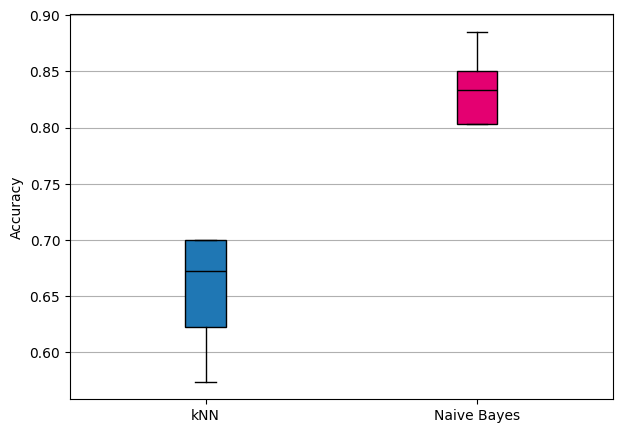
\includegraphics[width=12cm]{./Part II/1_a.png}
          \caption{Boxplot of the fold accuracies for each classifier}
    \end{figure}

\vspace{20pt}


\textbf{b. Report the accuracy of both models, this time scaling the data with a
Min-Max scaler before training the models. Explain the impact that this
preprocessing step has on the performance of each model, providing an
explanation for the results.}

\vspace{20pt}
\lstinputlisting[language=Python]{./Part II/1_b.py}

\begin{figure}[H]
    \centering
      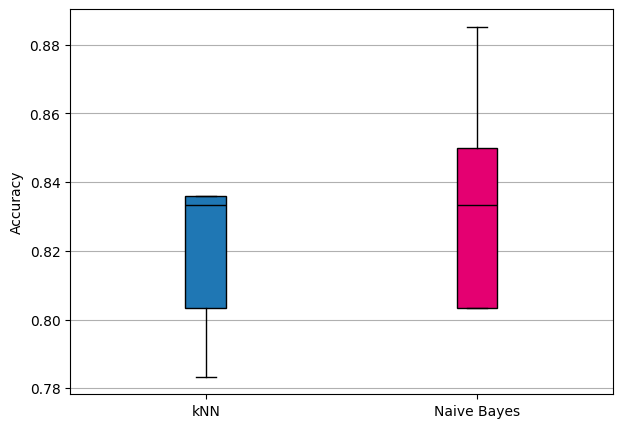
\includegraphics[width=12cm]{./Part II/1_b.png}
      \caption{Accuracy of both models with Min-Max scaling}
\end{figure}

\vspace{20pt}
\textbf{c. Using scipy, test the hypothesis "the $\mathbf{kNN}$ model is statistically superior to naive Bayes regarding accuracy", asserting whether it is true.}

\vspace{20pt}
\textbf{(2) a 80-20 train-test split, vary the number of neighbors of a $\mathbf{kNN}$ classifier using $\mathbf{k=\{1, 5, 10, 20, 30\}}$. Additionally, for each $k$, train one classifier using uniform weights and distance weights.}

\vspace{10pt}
\textbf{a. Plot the train and test accuracy for each model}

\vspace{20pt}
\lstinputlisting[language=Python]{./Part II/2_a.py}

\begin{figure}[H]
    \centering
      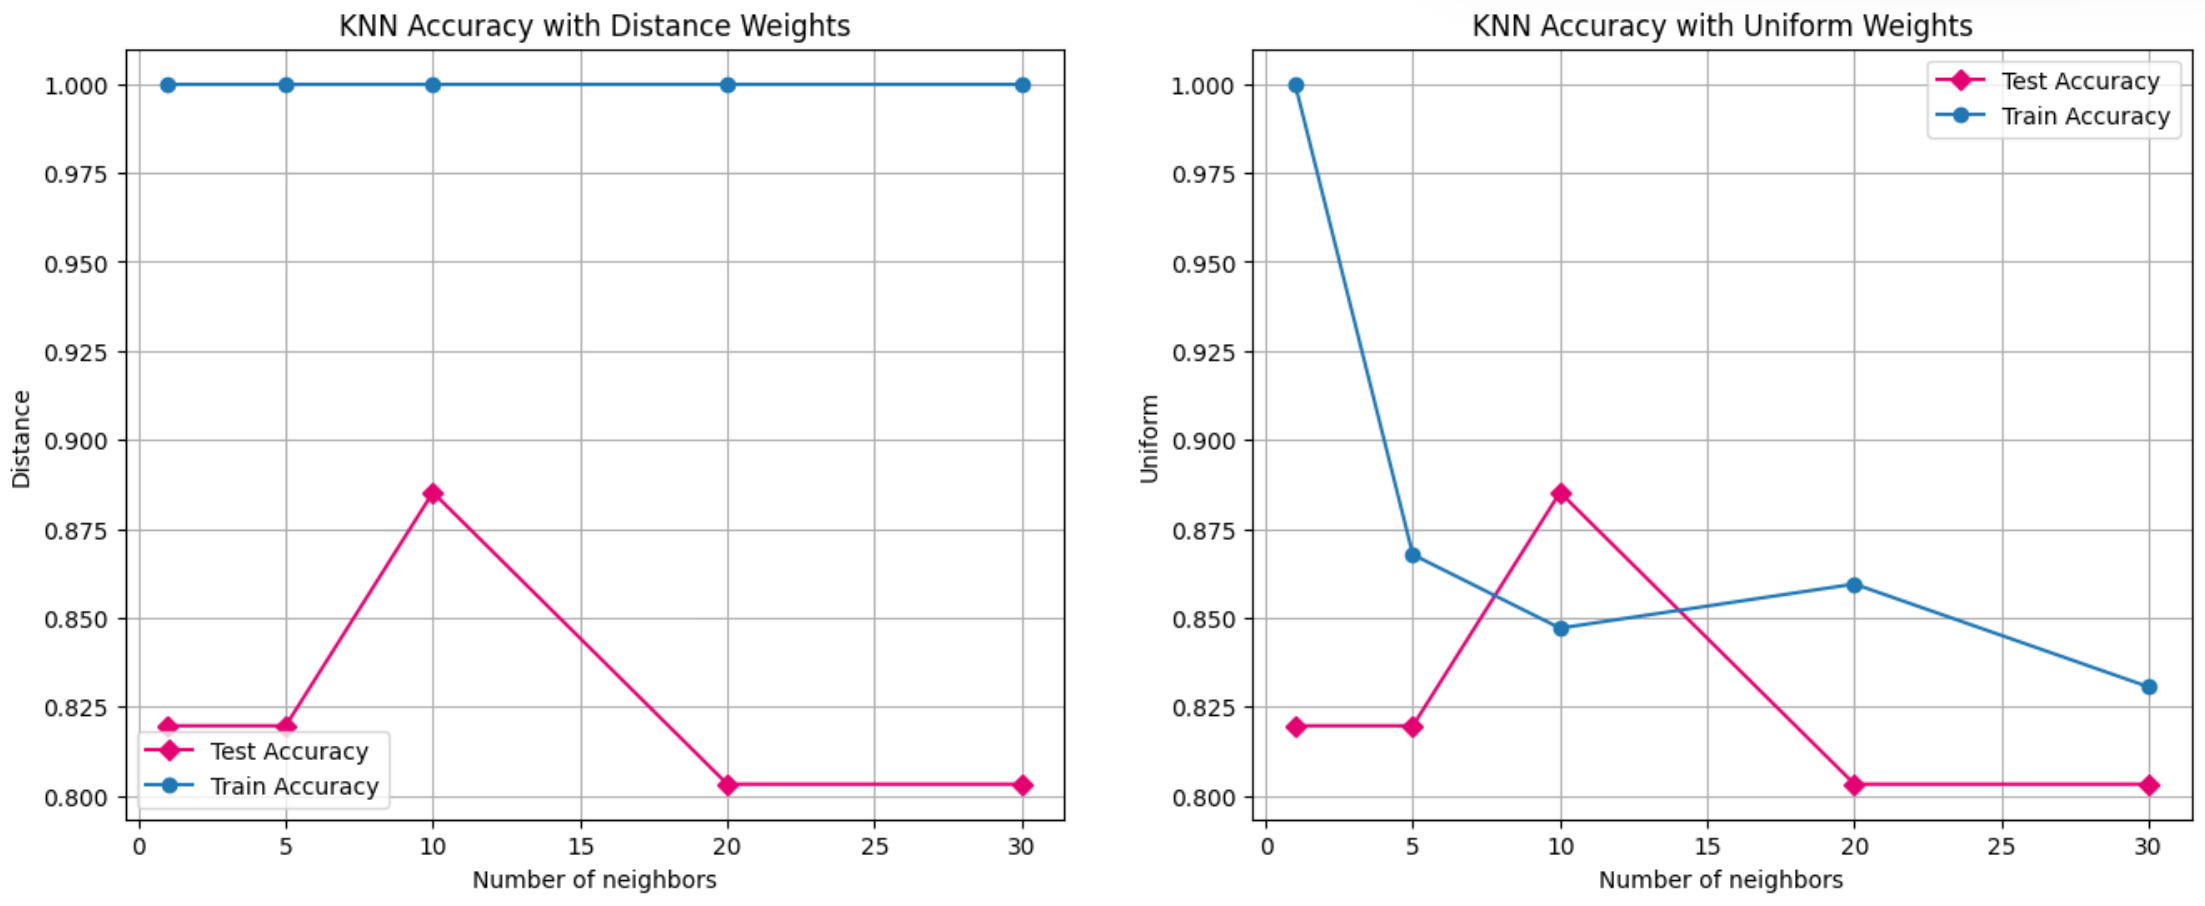
\includegraphics[width=12cm]{./Part II/2_a.png}
      \caption{Train and test accuracy for each model}
\end{figure}

\vspace{20pt}
\textbf{b. Explain the impact of increasing the neighbors on the generalization ability of the models.}

\vspace{20pt}
\textbf{(3) Considering the unique properties of the heart-disease.csv dataset, identify two
possible difficulties of the naïve Bayes model used in the previous exercises when learning
from the given dataset.}





\end{document}
